% !TEX root=/home/tavant/these/manuscript/src/manuscript.tex

% \FloatBarrier

\section{Comparison of the sheath model with PIC simulations} \label{subsec-picandmodel}

  % \begin{figure}[hbtp]
  %   \centering
  %   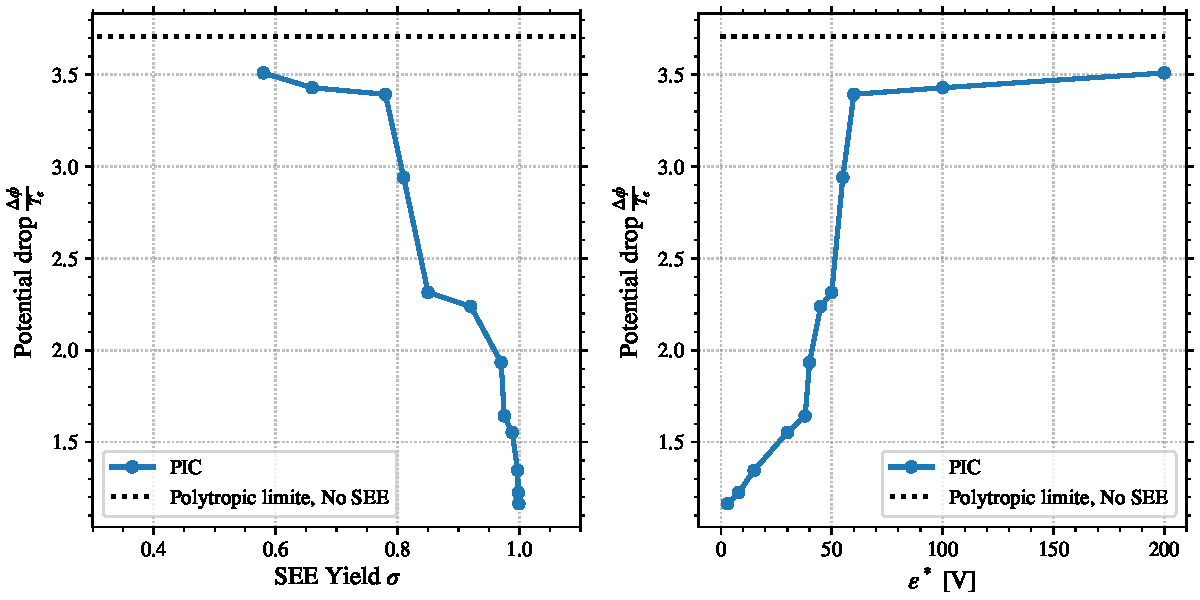
\includegraphics[width=\textwidth]{dphi_polytropic_noSEE}
  %   \caption{PIC simulation results (with SEE) compared to the polytropic limit without SEE.}
  %   \label{fig-polytropic_pic_noSEE}
  % \end{figure}
  % 
  % \begin{figure}[hbtp]
  %   \centering
  %   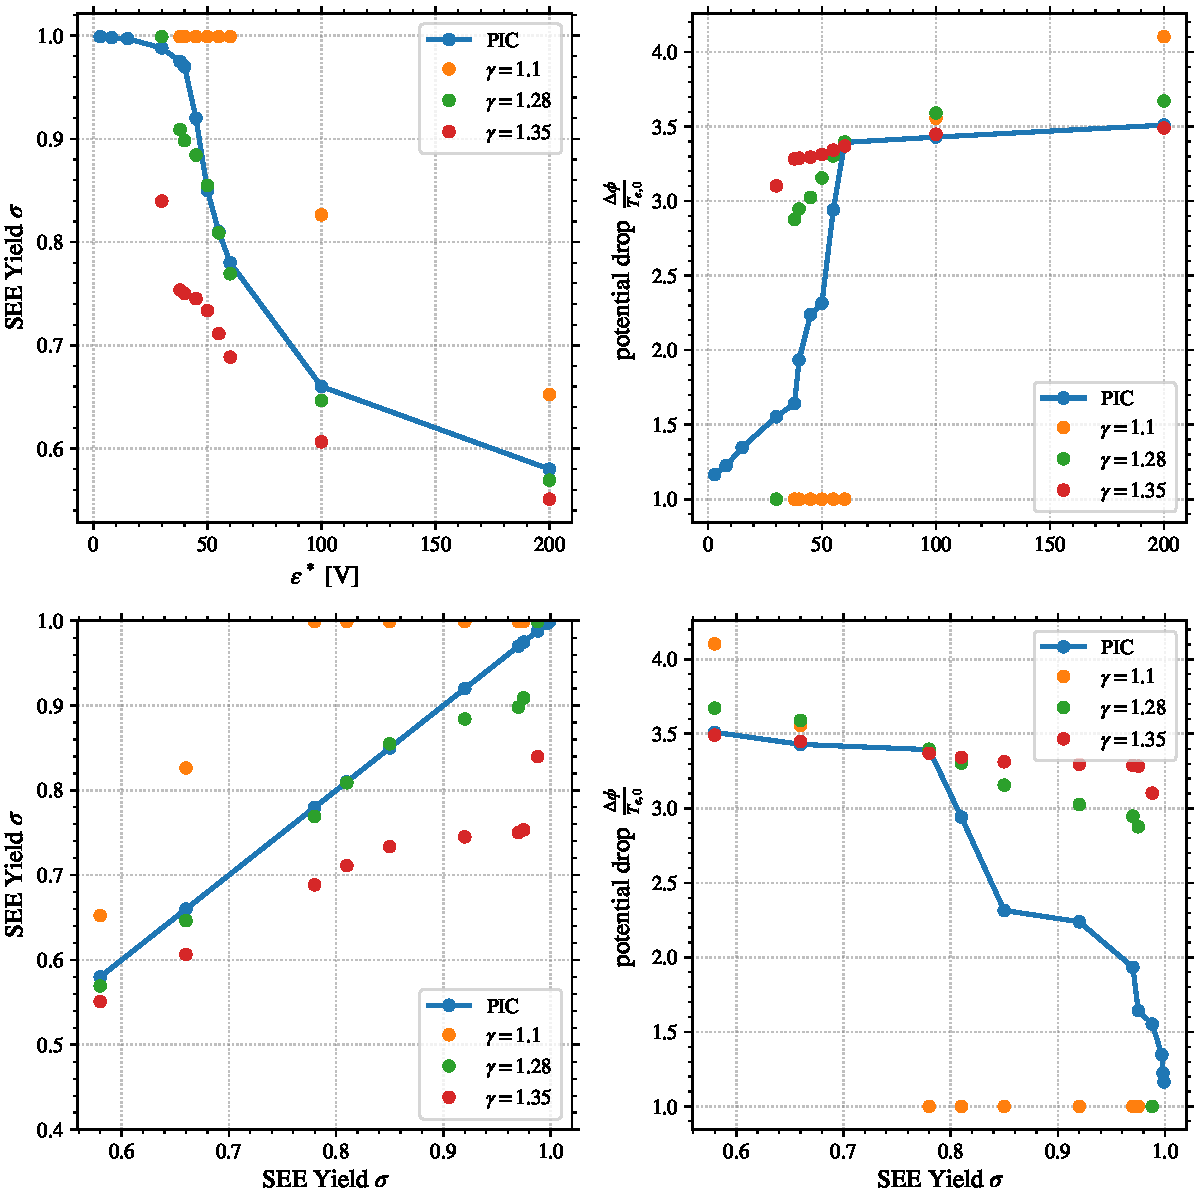
\includegraphics[width=\textwidth]{Summary_polytropic_SEE.pdf}
  %   \caption{Comparison of the PIC simulation results with the polytropic model with SEE.}
  %   \label{fig-polytropic_see_summary}
  % \end{figure}

  We compare in this section the characteristics of the plasma wall interaction observed in the \ac{PIC} simulations with the fluid model developed in \cref{sec-fluid_poly_see}.
  We first compare the mean values using in the parametric study over the crossover energy $\crover$, then we investigate the oscillation of regime {\bf II}.

  \subsection{Parametric study of the modified sheath model} \label{subsec-param_sheath_see}

    The variables of interest to characterize the plasma-wall interaction are the averaged electron emission rate $\rate$ and the plasma potential drop to the wall.
    The only input of the model is the electron mean temperature in the bulk $\Teb$, as well as the polytropic index $\gamma$.
    As seen in \cref{sec-PIC_poly}, the polytropic index of the electron population is measured in the \ac{PIC} simulation to $\gamma=1.35$.
    However, the electrons going toward the wall present a different index, measured from the bulk \ac{EVDF} to $\gamma=1.28$.
    These two values will be compared.

    Using the mean electron temperature measured in the simulation, we first compute the plasma potential drop $\dphi$ by solving \cref{eq-costseepoly} with $\gamma=1.35$.
    As showed in \cref{fig-rso_crit_see}, up to three solutions are possible.
    The emission rate $\rate$ is then computed using \cref{eq-seemaxw_Tew}, using the two values for $\gamma$.
    As discussed previously, the rate is limited to $\ratecr=0.982$ to take into account the \ac{SCL} regime.

    The results are shown in \Cref{fig-Poly_model_vs_pic}.
    The plasma potential drop computed is increased by $\Teb/2$ corresponding to the pre-sheath drop to better match the plasma potential measured in the simulations.
    \improvement{The Bhom criterion is slightly modified with the polytropic model, so it should not exactly be $\Teb/2$. however, it matches to well here that I do not really want to change !}

    \begin{figure}[hbtp]
      \centering
      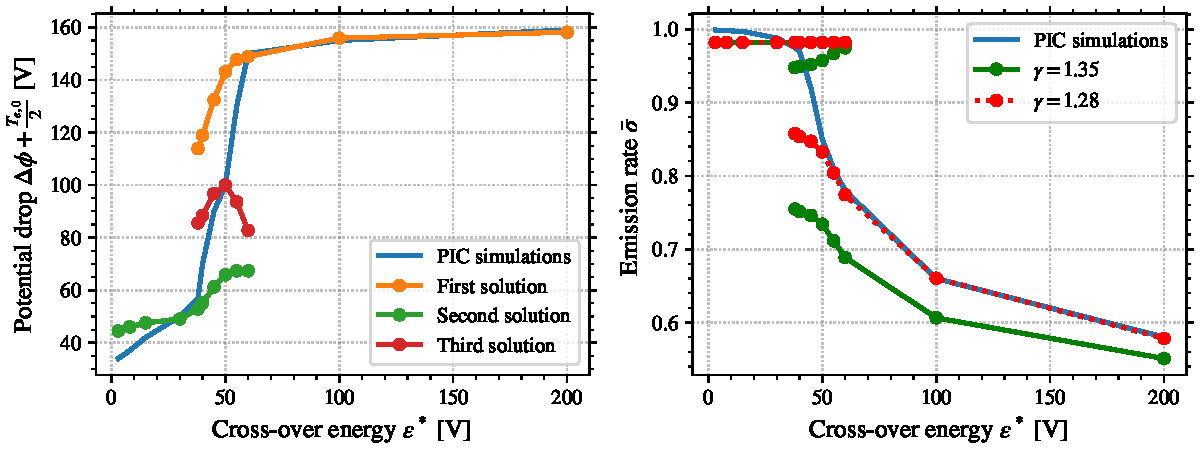
\includegraphics[width=\textwidth]{Poly_model_vs_pic}
      \caption{Comparison of the PIC simulations and the sheath model for the plasma potential drop from the center to the wall and the electron emission yield. }
      \label{fig-Poly_model_vs_pic}
    \end{figure}

    Concerning $\dphi$, we can see that the sheath model combining the polytropic state law and the electron emission is in good agreement with the \ac{PIC} simulations.
    We can see that the region where the three solutions coexist corresponds well with the regime {\bf II}.

    Concerning the emission rate $\rate$, we observe that the value $\gamma=1.35$ under estimates $\rate$ compared to the values of the \ac{PIC} simulations.
    On the other hand, $\gamma=1.28$ is in very good agreement.
    Interestingly, the saturation of the mean electron emission rate in the \ac{PIC} simulation is greater than the critical value $\ratecr$.
    
    %\inlinenote{ As $\rate$ is better with $\gamma=1.28$, we should use both values in \cref{eq-costseepoly}. However, this increases the complexity the equations and the model, and add 1 more free parameters (they would be 2 values for $\gamma$ now). I can say that only in the discussion maybe ? }
    
  \subsection{Sheath oscillation of regime {\bf II}} \label{subsec-pic_scheath_RSO}
  
    The regime {\bf II} is characterized by the present of oscillations between two meta-stable regimes {\bf III} and {\bf I}, one with a low emissivity and the other with a high emissivity.
    \Cref{fig-long_time} shows the temporal evolution of the electron temperature and the plasma potential relative to the wall for $\crover=45\,\volt$.
    The electron temperature is computed over the whole electron population in the simulation.
    Both the radial temperature $\Te_{,R}$ and the total and averaged, temperature $\Te$ are shown.
    The plasma potential $\dphi$ showed is measured at the center of the radial direction of the simulation, averaged over the azimuthal direction.
    
    
    \begin{figure}[hbtp]
      \centering
      \begin{tabular}{c c}
        \subfigure{long_time_dphi}{a}{20,20} &
        \subfigure{long_time_Te}{b}{20,20} \\
      \end{tabular}
      \caption{Temporal evolution of ({\bf a}) the plasma potential $\dphi$ and ({\bf b}) the electron temperature.}
      \label{fig-long_time}
    \end{figure}
    
    We clearly see in \cref{fig-long_time} the quasi-periodic oscillations between the two states.
    We observed that the electron temperature is slightly anisotropic, with the radial temperature smaller than the axial temperature.
    This anisotropy observed was not taken into account in the sheath model.
    More precisely, the $\Te_{,R}$ is linked to the thermal flux of electron toward the wall, while the total temperature $\Te$ is used in the computation of the electron emission rate $\ratemaxw$.
    However, the degree of anisotropy is not very high, as it is of the order of 10\% when the sheath is not inverted.
    When the sheath is inverted, the anisotropy is of the order of 25\%, as the electron with a large radial energy are quickly absorbed.
    However in the state, we suppose that the electron emission rate saturates at $\rate=\ratecr$, hence the impact of the total energy is less important with respect of the radial energy.
    Hence, we will compare the prediction using only the radial temperature $\Te_{,R}$ or the total, averaged, temperature $\Te$, but not the two of them together.
    
    \Cref{fig-dphi_te_PIc} shows the potential drop as a function of the electron temperature measured in the \ac{PIC} simulation (same case as \cref{fig-long_time}).
    Is also shown the theoretical solutions obtained with the model of \cref{sec-fluid_poly_see} using a constant polytropic index $\gamma=1.35$ and $\crover=45\,\volt$.
    
    \begin{figure}[hbtp]
      \centering
      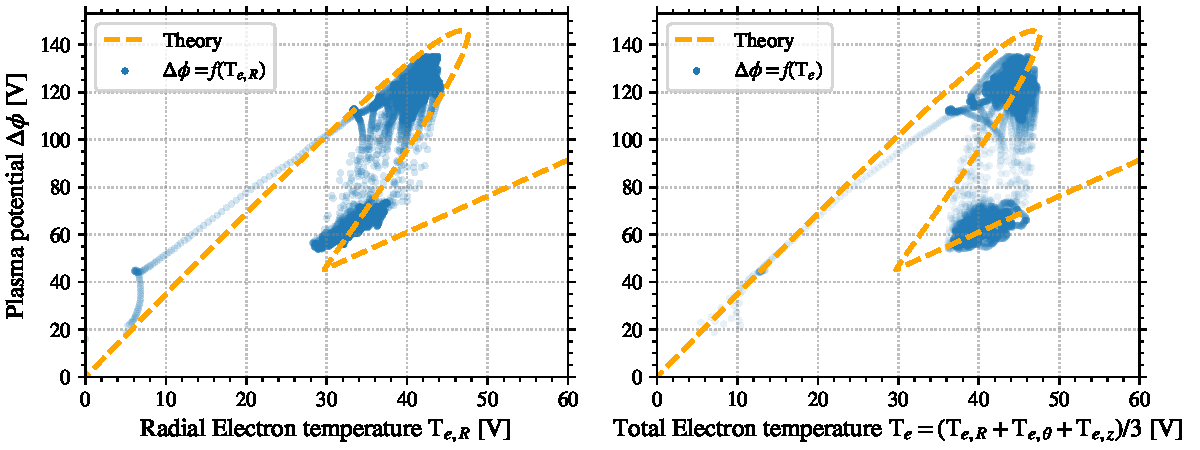
\includegraphics[width=\textwidth]{parametric_PIC_dphi_Te}
      \caption{Plasma potential as a function of (left) the radial electron temperature and (left) the total electron temperature. The blue markers represents the \ac{PIC} results presented in \cref{fig-long_time}, and the orange dashed lines correspond to the theoretical values with $\gamma=1.35$.}
      \label{fig-dphi_te_PIc}
    \end{figure}
    
    We can see in \cref{fig-dphi_te_PIc} that the sheath characteristics observed in the \ac{PIC}  simulations matches relatively well the theoretically values.
    In particular, we see the cohabitation of the two solutions of $\dphi$ observed for the same electron temperature, which corresponds to the domain of electron temperature for which the sheath model also predicts multiple solutions.
    
    During the state corresponding to regime {\bf III} (high value of  $\dphi$), the \ac{PIC} values are too noisy to clearly determine if the sheath follows the first or the second branch of the solutions.
    On the other hand, we see relatively well the correspondence betwee the \ac{PIC} results and the theory for the regime {\bf I} (low value of $\dphi$).
    
    As discussed previously, the value of the polytropic index, when computing by propagating the \ac{EVDF}, is $\gamma=1.28$.
    \Cref{fig-dphi_te_PIc2} is the same as \cref{fig-dphi_te_PIc}, but  the theoretical values of $\dphi$ using $\gamma=1.28$ is added.
    We can see that using the value $\gamma=1.28$ does not change significantly the value of the solution, except for the maximum value of the electron temperature for the first branch of the solutions, and the domain of temperature where the 3 solutions coexist.
    In the case of $\gamma=1.28$, the \ac{PIC} simulation result does not corresponds to the domain with the theoretical multiple solutions.
    
    \begin{figure}[hbtp]
      \centering
      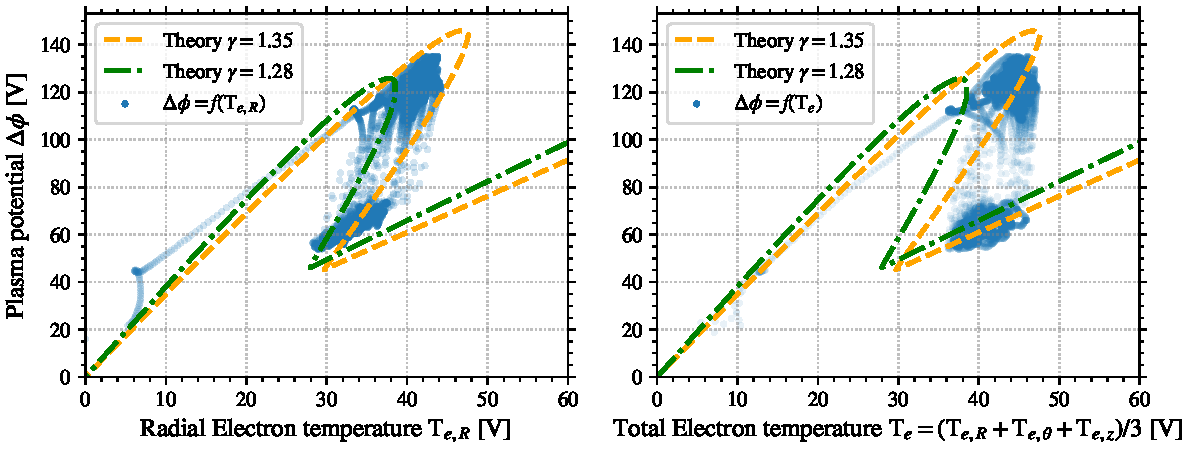
\includegraphics[width=\textwidth]{parametric_PIC_dphi_Te_two_gamma}
      \caption{Similarly to \cref{fig-dphi_te_PIc}, Plasma potential as a function of (left) the radial electron temperature and (left) the total electron temperature. The blue markers represents the \ac{PIC} results presented in \cref{fig-long_time}, the orange dashed lines correspond to the theoretical values with $\gamma=1.35$, and the green dotted-dashed line is computed with $\gamma=1.28$.}
      \label{fig-dphi_te_PIc2}
    \end{figure}
    
    One must note that the model are stationary, while the oscillations observed are relatively fast.
    Indeed, the ion dynamic is 
    \begin{equation} \label{eq-ti}
      \tau_i = \frac{2 \pi}{\opi} = 0.1 \,\micro\second
    \end{equation}
    
    \inlinenote{Ha bah en fait non ! Voir avec le temps pour le temps de formation de la pres-gaine via le time-of-flight des ions }
    
    The sheath oscillations of regime {\bf II} have been observed in \citet{croes2017} with three different ion masses: xenon, krypton and argon.
    The results are shown in \cref{fig-RSO_altern}.
    We can see that the period of the oscillations vary with the ion masses, indicating that it has a role in the dynamics of the oscillation.
    
    \begin{figure}[hbtp]
      \centering
      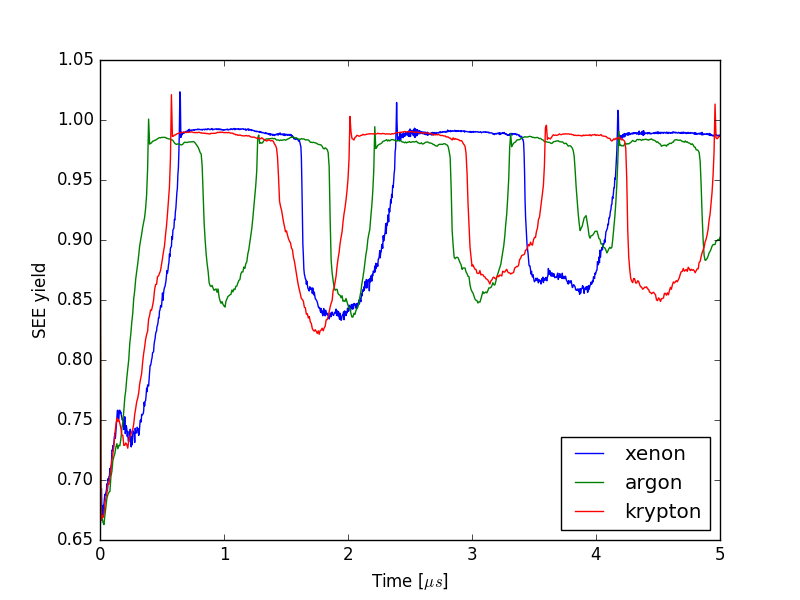
\includegraphics[width=\defaultwidth]{SEE_RSOs.png}
      \caption{Temporal evolution of the SEE rate $\rate$ measured in the PIC simulations for different gases (xenon, krypton, and argon), taken from \citet{croes2017}.}
      \label{fig-RSO_altern}
    \end{figure}
    
    \subsection{Theoretical values of the critical electron temperature} \label{subsec-theo_Tecr}
    
    In \cref{sec-fluid_poly_see}, \cref{eq-costseepoly} returns either one or three solutions.
    For two values of $\Te$, one of the solutions is double.
    This values, noted $\Te^1$ and $\Te^2$ corresponds to the theoretical threshold values for which the usual sheath regime and  the \ac{SCL} regime exist, respectively.
    
    \paragraph{Maximum electron temperature value, $\Te^1$\\}
    
    The first critical electron temperature  $\Te^1$  corresponds to the maximum temperature of the first branch (corresponding to regime {\bf III}).
    It correspond to the solution of \cref{eq-costseepoly} that is also a solution of its derivative with respect to $\chi$.
    Once again, the equation is not trivial, and cannot be solved analytically.
    thus, we solve it numerically.

    \begin{figure}[hbtp]
      \centering
      \begin{tabular}{cc}
        \subfigure{Maximum_Te1_epsilon.pdf}{a}{20,20} &
        \subfigure{Maximum_Te1_gamma.pdf}{b}{20,15} \\
      \end{tabular}
      \caption{Variation of $\Te^1$ as a function of ({\bf a}) $\crover$ for two values of $\gamma$, and ({\bf b}) $\gamma$ for two values of $\crover$.}
      \label{fig-Te1_epsi}
    \end{figure}
    
    \Cref{fig-Te1_epsi} shows the variation of $\Te^1$ as a function of   $\crover$  and $\gamma$.
    We can see that the maximum temperature $Te^1$ increases linearly with $\crover$.
    This was expected, as in \cref{eq-costseepoly}, the only time that $\Teb$ is explicitly present is in the therm $\frac{\Teb}{\crover}$.
    On the other hand, the variation with $\gamma$ follows a power law, monotonically increasing.
    The values observed correspond well with the theoretical values showed in \cref{fig-dphi_te_PIc2}.
    
    In \citet{raitses2006}, the authors compare the maximum of the axial profile of the electron temperature $\hat{\Te}$ measured in a \ac{HET} with two different wall material, once with a very low emissivity carbon velvet material, the other the conventional \ac{BN} ceramic.
    \Cref{fig-raiteses2006} reproduces the results obtained in \citet{raitses2006}.
    
    \begin{figure}[hbtp]
      \centering
      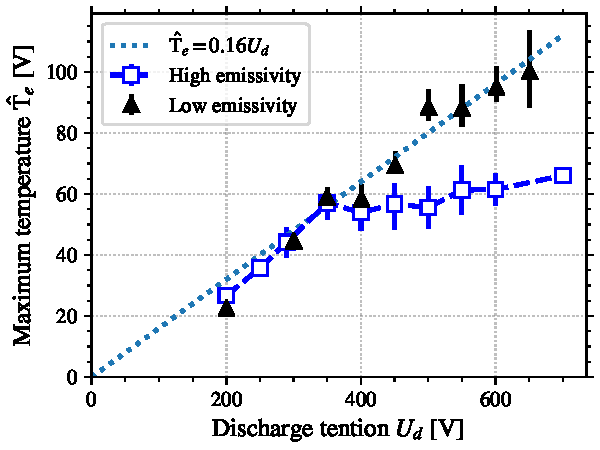
\includegraphics[width=\defaultwidth]{Raiteses_remaked.pdf}
      \caption{ The dependence of the maximum electron temperature on the discharge  voltage for a conventional thruster with high-SEE ac{BN} channel walls and the segmented thruster with low-SEE floating segmented electrodes made of carbon velvet material. Reproducibility of measurements is shown by error bars. Adapted from \citet[Fig. 3]{raitses2006} }
      \label{fig-raiteses2006}
    \end{figure}
    
    
    They observed that with the ceramic, the values of $\hat{\Te}$ present a maximum value that cannot be exceed, while the results with the low emissivity material does not present such maximum.
    The maximum value of $\hat{\Te}$ measured is $\hat{\Te}^1 = 55 \pm 6\,\volt$, the error correspond to reproducibility of the measurements (manually extracted from \citep[Fig. 3]{raitses2006}, reproduced in \cref{fig-raiteses2006}).
    For a \ac{BN} wall, we have $\crover\simeq 35\,\volt$ \citet{smirnov2004}.
    This value is higher than the value observed in the \ac{PIC} simulation and obtained with the sheath model, but the agreement is significantly better than the isothermal sheath model prediction 
    \begin{equation} \label{eq-Temaxisothermal}
      \Te^1_{\rm , isothermal} \simeq \frac{\crover}{2} \simeq 17.5 \,\volt.
    \end{equation}
    
    
    \paragraph{Minimum electron temperature value for regime {\bf I}, $\Te^2$\\}
    
    The minimum electron temperature value for regime {\bf I}, $\Te^2$, corresponds to the case where the electron temperature at the wall induces an emission rate $\ratemaxw (\Tew) = \ratecr$.
    Noting $C_1 = \frac{\ratecr - \sigo}{1-\sigo} = 0.964$, we obtain
    \begin{equation} \label{eq-Te2}
      (1-\ratecr) \lp 2 - \frac{C_1 \crover}{2 \Te^2} \rp^{\frac{1}{(\gamma-1)}} \sqrt{\frac{C_1 \crover}{2 \Te^2}} = \sqrt{\frac{4 \gamma \pi m_e}{m_i}}
    \end{equation}
    
    \Cref{eq-Te2} is solved numerically.
    The solutions for different values of $\crover$ and $\gamma$ are shown in \cref{fig-Te2_epsi}.
    Interestingly, the minimum temperature $\Te^2$ now decreases with the value of $\gamma$.
    Hence, the sheath can stay in the \ac{SCL} regime at a lower electron bulk temperature $\Teb$ than predicted with the isothermal hypothesis.
    
    \begin{figure}[hbtp]
      \centering
      \begin{tabular}{cc}
        \subfigure{Maximum_Te2_epsilon.pdf}{a}{20,25} &
        \subfigure{Maximum_Te2_gamma.pdf}{b}{20,20} \\
      \end{tabular}
      \caption{Variation of $\Te^2$ as a function of ({\bf a}) $\crover$ for two values of $\gamma$, and ({\bf b}) $\gamma$ for two values of $\crover$.}
      \label{fig-Te2_epsi}
    \end{figure}
    
    